\documentclass{llncs}
\usepackage{graphicx}
\usepackage{amsmath}
\usepackage{amssymb}
\usepackage{algorithm}
\usepackage[noend]{algpseudocode}

\begin{document}
\mainmatter  % start of an individual contribution
\pagestyle{empty}

\title{Low-cost IoT, Big Data, and Cloud Platform for Developing Countries}

\author{Corentin Dupont\inst{1}, Tomas Bures\inst{2}, Mehdi Sheikhalishahi\inst{2}, Congduc Pham\inst{3}, Abdur Rahim\inst{1}}		 
\institute{FBK/Create-Net\\
\email{cdupont@fbk.eu,arahim@fbk.eu}
\and
Innotec21 GmbH\\
\email{mehdi.sheikhalishahi@innotec21.de,tomas.bures@innotec21.de}
\and
University of Pau\\
\email{congduc.pham@univ-pau.fr}
}

\maketitle

\begin{abstract}
Gartner forecasts that 6.4 billion connected things will be in use worldwide in 2016, up 30 percent from 2015, and will reach 20.8 billion by 2020.
In 2016, 5.5 million new things will get connected every day.
Furthermore, the current research  and marker trends shows the convergence between IoT and Big Data.
On the other hand, developing countries are still far from being able to benefit from IoT infrastructures.
In this paper we explain how IoT can be made available for everybody and we present WAZIUP, a project aiming at building an open innovation platform able to accelerate innovation in developing countries and rural areas.
The WAZIUP IoT platform will allow the development of IoT applications coupled with Big Data capabilities.
The platform is tailored to the specific requirements and constraints of developing countries.
We will give an overview of the WAZIUP IoT and Big Data platform and then detail its technical aspects.

\end{abstract}

\keywords{IoT, Big Data, Low-cost IoT platform, Cloud Computing}

%
\section{Introduction}

\todo{change this intro to fit paper objectives: low cost HW review, Security/AuthN/AuthZ, data analytics using Elastic search, market opportunities}

\noindent
\todo{C. Pham: the idea is to say that there will be a huge uptake of IoT devices that will be deployed worldwide for a large variety of applications; and that needs suitable platforms. This uptake will definitely come from the possibility and the availability of low-cost IoT devices that can be deployed in a very simple manner thanks to new radio technologies.}

ICT developments in Africa has already enabled significant modernizations across traditional sectors.
Notable examples are the micro-health insurance accessible through mobile devices, index-based crop insurance and crowd-sourced management of public services.
These innovative applications recognize and leverage commonalities between sectors, blur traditional lines, and open up a new field of opportunities.

The opportunity for ICT in Africa is huge especially for IoT and big data: those technologies are promising a big wave of innovation for our daily lives.
The promise of IoT is to connect billions of sensors, devices, equipment and systems.
In turn, the challenge is to drive business outcomes, consumer benefits, and to create new value.
The new mantras for the IoT Era is the collection, convergence and exploitation of data.
The information is collected from sensors, devices, gateways, edge equipment and networks and stored in their respective IoT platforms.
This information is processed in order to increase business efficiency through automation while reducing downtime and improving people productivity.

While developed countries are discussing about massive deployment of IoT, countries in Sub-Saharan Africa are still far from being ready to enjoy the full benefit of Iot.
They face many challenges, such as the lack of infrastructure and the high cost platforms complexity in deployment.
At the same time, it is urgent to promote IoT worldwide : WAZIUP will contribute by reducing part of the technology gap between EU and Africa.
The goal of WAZIUP is to deploy an IoT and big data platform for African needs and validate it through several Sub Saharan Africa real-life use cases.

WAZIUP targets the rural community in Sub-Saharan Africa: about 64\% of the population is living outside cities.
The region will be predominantly rural for at least another generation.
The pace of urbanization here is slower compared to other continents, and the rural population is expected to grow until 2045.
The majority of rural residents live on less than few euros per day.
Rural development is particularly imperative in sub-Saharan Africa, where half of the rural people depends on the agriculture/micro and small farm business, other half faces rare formal employment and pervasive unemployment.
For rural development, technologies have to support several key application sectors such as living quality, health, agriculture and climate changes.

The biggest challenge of WAZIUP is to reduce costs and power consumption while increasing the robustness of the hardware.
Hardware has to be robust enough so as to require lower maintenance and handle environmental and deployment treats as well.
WAZIUP will present an innovative design of the IoT platform dedicated to the rural ecosystem.
To achieve that, low-cost, generic building blocks will be deployed for maximum adaptation to end-applications in the context of the rural economy in developing countries.
Another challenge of WAZIUP is to be able to manage the network deployment and to facilitate IoT communication.
Lower cost solutions has to be used : privilege price and single hop dedicated communication networks, energy autonomous, with low maintenance costs and long lasting operations.
Dynamic management of long range connectivity has to be taken into account (e.g., cope with network \& service fluctuations), such as devices identification, abstraction/virtualization of devices, communication and network resources optimization.
Finally, WAZIUP aims to exploit the potential of big-data applications in the specific rural context.
Data will be collected from the IoT sensors themselves, but WAZIUP will also collect open data from other sources to build predictive models and enrich the platform.

From a technical standpoint, WAZIUP will pay attention to all related privacy and security aspects with specifics addressing the involved communities such as farmers, and developers.

Continued Openness will be ensured through the release of open specification and open software components and/or algorithms.
Low-cost and low-energy consumption will be possible through the design of innovation hardware (sensors/actuators), and of IoT communication \& network infrastructure.

The challenges outlined above will be tackled using an open IoT-Big Data Platform with affordable sensors connected through an Iot-Cloud open platform. 
The technical functionalities encompassed by the platform will be a cloud-based real-time data collection combined with analytics and automation software, an intelligent analytics of sensor and device data, an integration to third parties platforms and a Platform-as-a-Service (PaaS) provider.

The PaaS will provide to business clientele with independently maintained platform upon which their web application, services and mobile applications can be built. 

The rest of this paper is structured as follows: Section~\ref{sec:platform} presents the architecture of the WAZIUP platform. 
Section~\ref{sec:implem} shows the implementation chosen. 
Section~\ref{sec:deploy} details the deployement of WAZIUP, contrained by its environment.
Section~\ref{sec:usecases} presents four use cases that will be used to validate the WAZIUP concepts.
Section~\ref{sec:relworks} presents a survey of the literature on the topic, together with a survey of the Big Data Open Source tools.
Finally we conclude the chapter in Section~\ref{sec:conclu}.

\section{Introduction}

ICT developments in developing countries has the potential to cut across traditional sectors: notable examples are the introduction of micro-health insurance and health-savings accounts through mobile devices; index-based crop insurance; crowd-sourcing to monitor and manage the delivery of public services.
These innovative applications recognize and leverage commonalities between sectors, blur traditional lines, and open up a new field of opportunities.
The opportunity for ICT intervention in developing countries is huge especially for IoT and big data: those technologies are promising a big wave of innovation for our daily life \cite{Sarkar2016,ITU2015}.


The era of IoT can connect a large variety of sensors, devices, equipment, systems.
In turn, the challenge is about driving business outcomes, consumer benefits, and the creation of new value.
The new mantras for the IoT era is the collection, convergence and exploitation of data.
The information collection involves data from sensors, devices, gateways, edge equipment and networks.
This information allows  increasing process efficiency through automation while reducing downtime and improving people productivity.
Figure \ref{figure-AfricaICTApp} shows some typical applications where remote monitoring facilities could greatly increase quality and productivity in a large variety of rural applications.


\begin{figure}[H]  
\centering  
\includegraphics[width=.6\linewidth]{figures/AfricaICTApp}  
\caption{Some ICT fields of IoT opportunities in rural environments}   
\label{figure-AfricaICTApp}  
\end{figure}

\vspace{-0.5cm}
However, developing countries are facing many difficulties -- lack of infrastructure, high cost of hardware, complexity in deployment, lack of technological eco-system and background, etc -- when it comes to real deployment of IoT solutions \cite{IoT-newletter-zennaro}, especially in remote and rural areas.
In this context, IoT deployment must address four major issues: (a) Longer range for rural access, (b) Cost of hardware and services, (c) Limit dependancy to proprietary infrastructures and (d) Provide local interaction models.


In this article, we present in Section \ref{iot} the new technologies and trends contributing in making IoT available at a much lower cost for worldwide adoption.
Then, we present in Section \ref{platform} the EU H2020 WAZIUP IoT platform targeting deployment of low-cost IoT and Big Data in developing countries, addressing the aforementioned major issues.
Section \ref{sec:conclu} concludes the article.


%\section{The IoT era with low-cost IoT for all}

\subsection{IoT connectivity made easy}

Recent Low-Power Wide Area Networks (LPWAN) technologies for Internet-of-Things (IoT) introduced by Sigfox and Semtech's (LoRa\texttrademark) are currently gaining incredible interest and are under intense deployment campaigns worldwide. They definitely initiated a new innovation cycle as they obviously provide a much better connectivity answer for IoT (most of IoT devices have small amount to data to send and very limited battery power) compared to traditional cellular-based connectivity (e.g. GSM/GPRS/3G) or short-range technologies such as IEEE 802.15.4. They offer several kilometers range without relay nodes to reach a central gateway, thus greatly simplifying large-scale deployment of IoT devices as opposed to the complex multi-hop approach needed by short-range radio technologies. Fig. \ref{figure-1hop} shows a typical extreme long-range 1-hop connectivity scenario to a long-range gateway, which is the single interface to Internet servers, using low-cost LoRa radio modules available from many vendors. Most of these long-range technologies can achieve 20km or higher range in line-of-sight (LOS) condition and about 2km-4km in non-LOS conditions \cite{semtech-test,Libelium-lora-web} such as in dense urban/city environments.

\begin{figure}[htb]  
\centering  
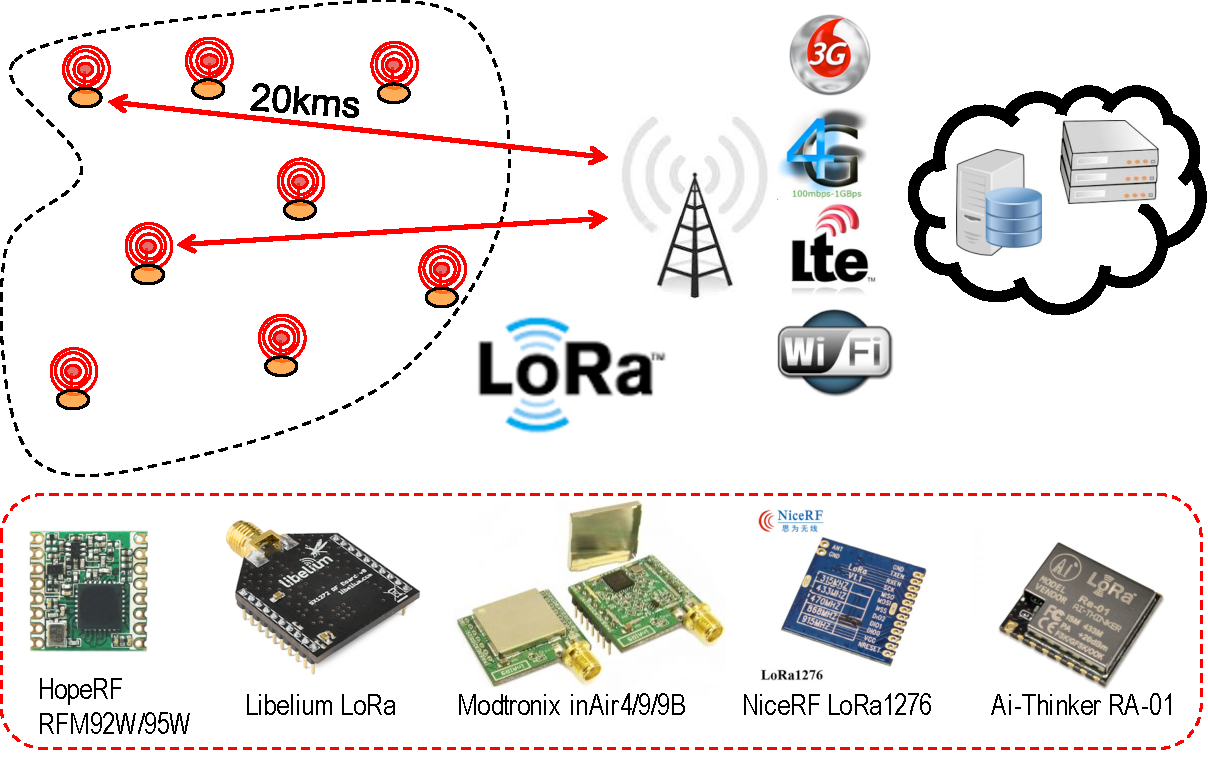
\includegraphics[width=.6\linewidth]{figures/1-hop}   
\caption{Extreme long-range application with new radio technologies}   
\label{figure-1hop}  
\end{figure} 

\subsection{Low-cost DIY IoT hardware}

Commercial IoT devices are getting mature but they are definitely too expensive for very low-income countries. In addition, these highly integrated devices are difficult to repair with their parts being hardly locally replaced.  The availability of low-cost, open-source hardware platforms such as Arduino boards definitely pushes for a Do-It-Yourself (DIY) and "off-the-shelves" design approach for a large variety of IoT applications. The Arduino ecosystem is large and proposes various board models, from large and powerful prototyping boards to smaller and less energy-consuming boards for final integration purposes as illustrated in Figure \ref{figure-generic-iot}. For instance, the small form factor Arduino Pro Mini board based on an ATmega328 microcontroller has a high performance/price tradeoff and can be used to build a low-cost generic sensing IoT platform with LoRa long-range transmission capability for about 7 euro: 2 euro for the Arduino and 5 euro for the radio module!

\begin{figure}  
\centering  
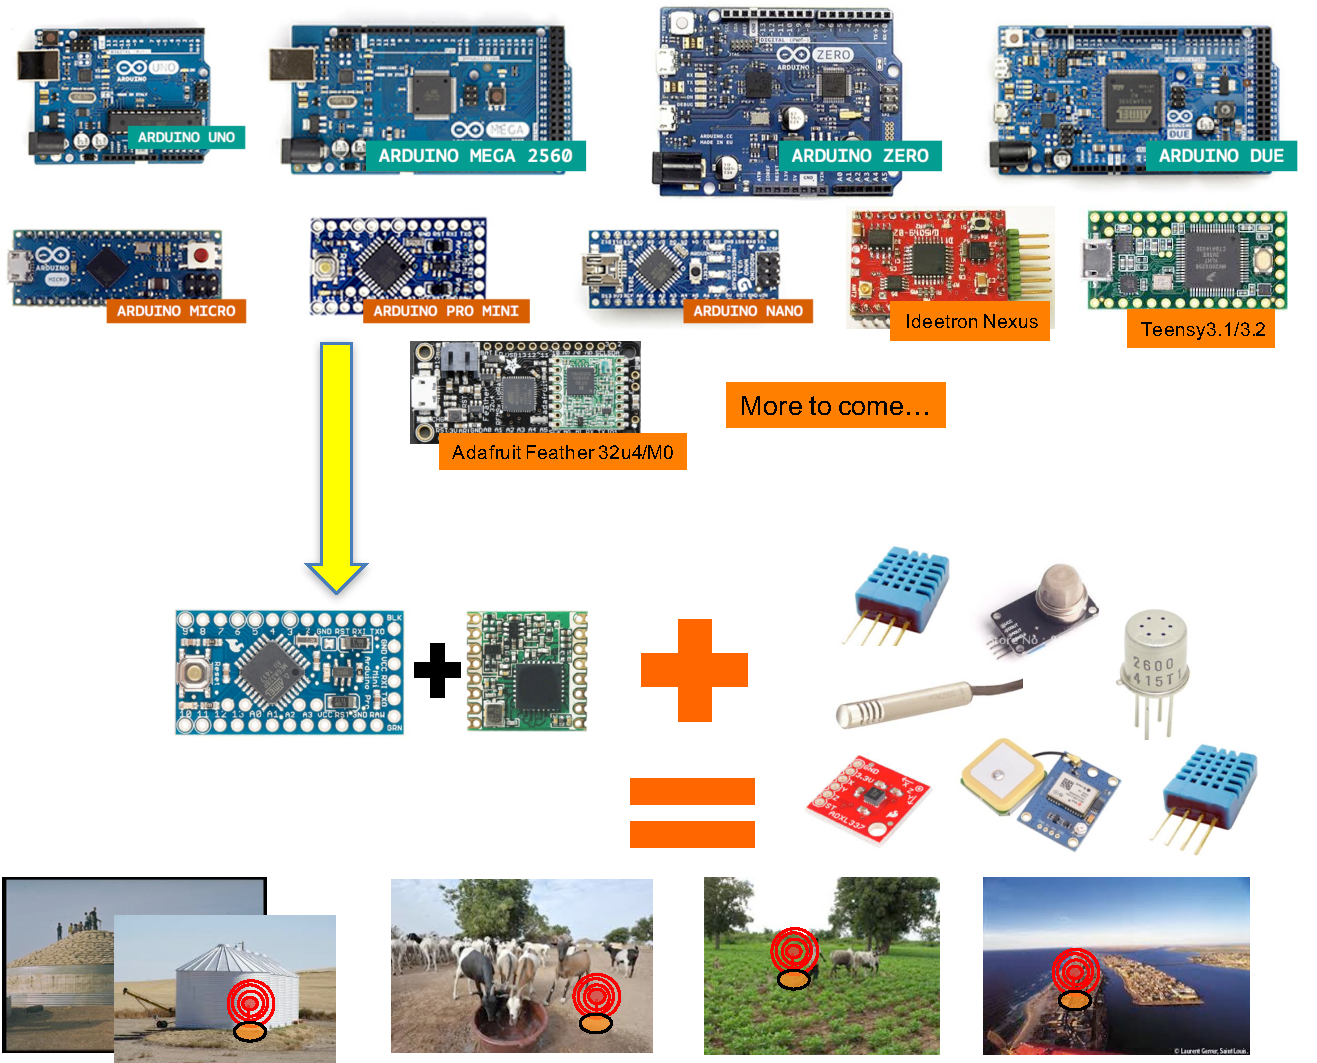
\includegraphics[width=.75\linewidth]{figures/generic-iot}   
\caption{Generic low-cost IoT hardware}   
\label{figure-generic-iot}  
\end{figure} 

Integration of these generic IoT becomes straightforward and the Arduino Pro Mini is available in the 3.3v \& 8MHz version for much lower power consumption, offering the possibility of running for more than a year on 4 AA regular batteries as illustrated in Fig. \ref{figure-easy-integration}. 

\begin{figure} 
\centering  
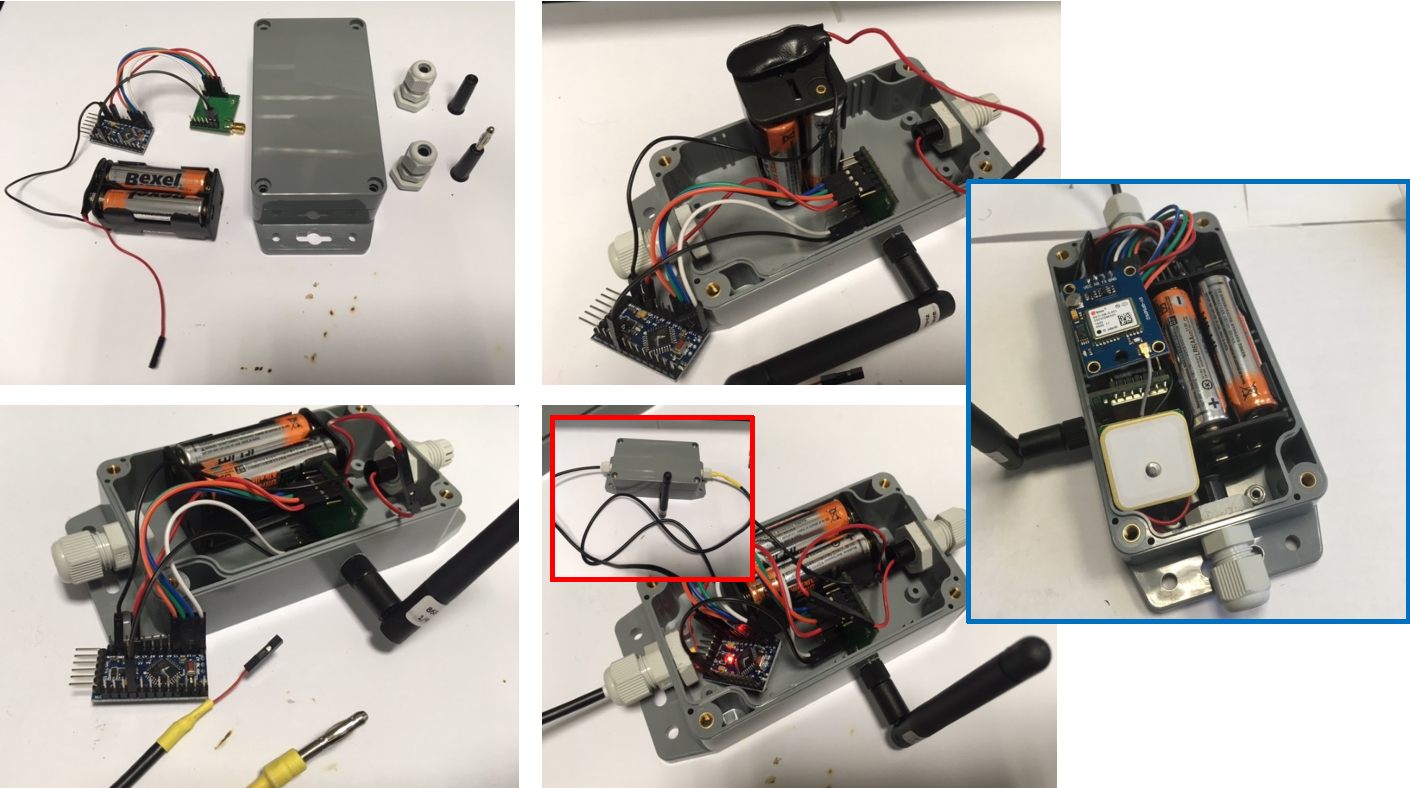
\includegraphics[width=.8\linewidth]{figures/easy-integration}   
\caption{Easy integration with DIY approach for maximum appropriation}   
\label{figure-easy-integration}  
\end{figure} 

It is expected that this availability of low-cost DIY IoT will create a tremendous uptake of the technology on a large-scale, for a large variety of applications, including those from developing countries as even a limited deployment of IoT devices can have huge impacts.

\subsection{Hardware and Software Security}
In a large scale IoT platform, that consists of local and global clouds, providing security is a challenge. A local cloud is connected to one or several IoT gateways that are close to local cloud. 

An IoT gateway is a wireless based on 4G/3G communications; thus, we cannot build a local/private network space with Local Cloud even. Somehow we need to have a public endpoint to access Orion from the Internet. Therefore, even in local cloud model we need a public endpoint. Even in local cloud model, we need a public IP or the IoT gateway would have to be in the local network.
In our platform, global cloud provides the main data broker (global Orion context broker) which receives data from distributed IoT gateways. IoT gateway communications with global Orion need to pass through the Internet. If Orion is exposed to the outside world using a public IP address of platform, then all access to Orion have to be controled in such a way to allow only authorized accesses, and deny non-authorized ones.

One way to provide security for such a communication is to use FIREWALL, and allow IP addresses of IoT gateways to be able to access Orion endpoint (e.g. public IP of platform: Orion Port). And then, deny all other accesses to Orion. Since we know that which IoT gateways are connected, or would like to connect to our platform this is a solution. At the end, we are enforcing access control to Orion by design with this solution. However, one issue can come from gateway with Internet access through a 3G dongle where the IP address is not always the same, and it may change. 

Generally, we can distinguish two scenarios for local cloud:
\begin{itemize}

\item 1) Connected with limited bandwidth (typically charged by transmitted data): Here we use local cloud to optimize for data usage because connecting to internet is expensive and slow. Data are transferred to local cloud from internet, but that's low amount compared to what would be needed to access the dashboard remotely. Here the local cloud need a public IP or we will have to implement a method to circumvent NATs. This would mean the local cloud periodically pull the data from global cloud with static public IP or it keeps an open connection to a cloud with static public IP. Data go from the IoT gateway to the global cloud and from there to the local cloud.

\item 2) Disconnected IoT gateway: In this case, the gateway must be connected with some local communication means (e.g. wifi, ethernet or LoRA) to the local network of the local cloud.
\end{itemize}

Therefore, it is important to have a co-design from hardware and software experts in place in order to address different scenarios.

Relying on IP address is not really good in some cases. There is another way in which we can rely in defining gateway id, and accepting only upload from registered gateways. It is easy to add a field in the message, to have the gateway id; thus, we can define access policies based on registered Gateway ids. For that, at platform, we need to receive the message, decode it and see if it is from a registered gateway id to let the communication happen. For this case, Gateway ID plus secure token sounds good for simple security. Alternatively, we could go for certificates. This would go nicely with securing the communication to go over SSL. To be sufficiently secure, we should communicate over HTTPS and use certificates. Since an IoT gateway is a Linux machine, we can certainly do the certificates and HTTPS.

This would mean that we have our own Certification Authority (CA). From this, we would generate certificates for the Orion and the gateway. Then we would setup both the parties to require that the opposite party presents a certificate signed by the CA.

This would have two benefits: 1) proper authentication, and 2) securing data during transport.
\section{Entering the IoT era}
\label{iot}

\subsection{IoT connectivity made easy}

Recent Low-Power Wide Area Networks (LPWAN) technologies for Internet-of-Things (IoT) introduced by Sigfox and Semtech's (LoRa\texttrademark) \cite{semtech-lora} are currently gaining incredible interest and are under intense deployment campaigns worldwide.
They definitely initiated a new innovation cycle as they obviously provide a much better connectivity answer for IoT (most of IoT devices have small amount to data to send and very limited battery power) compared to traditional cellular-based connectivity (e.g.
GSM/GPRS/3G) or short-range technologies such as IEEE 802.15.4.
They offer several kilometers range without relay nodes to reach a central gateway, thus greatly simplifying large-scale deployment of IoT devices as opposed to the complex multi-hop approach needed by short-range radio technologies.
Figure \ref{figure-1hop} shows a typical extreme long-range 1-hop connectivity scenario to a long-range gateway, which is the single interface to Internet servers, using low-cost LoRa radio modules available from many vendors.
Most of these long-range technologies can achieve 20km or higher range in line-of-sight (LOS) condition and about 2km-4km in non-LOS conditions \cite{semtech-test,Libelium-lora-web} such as in dense urban/city environments.


\begin{figure}[H]  
\centering  
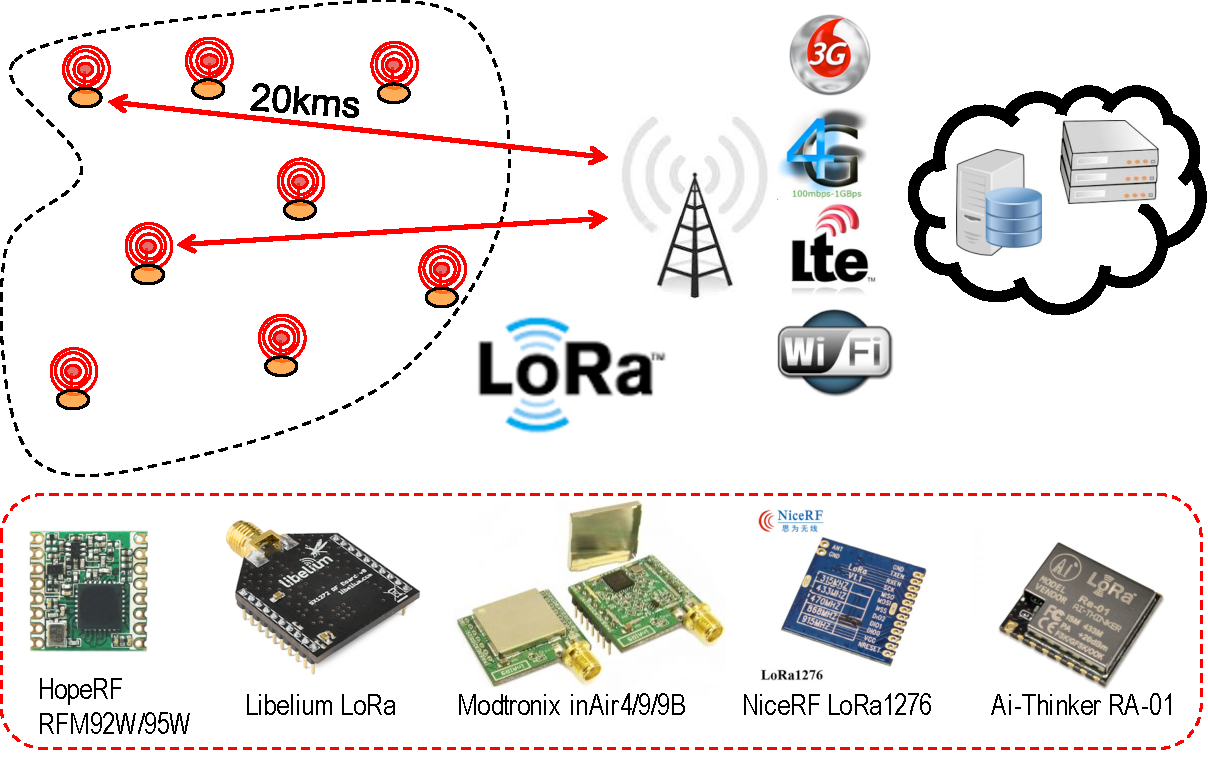
\includegraphics[width=.55\linewidth]{figures/1-hop}   
\caption{Extreme long-range application with new radio technologies}   
\label{figure-1hop}  
\end{figure} 

\vspace{-0.5cm}
\subsection{Low-cost DIY IoT hardware}

Commercial IoT devices are getting mature but they are definitely too expensive for very low-income countries.
In addition, these highly integrated devices are difficult to repair with their parts being hardly locally replaced.
The availability of low-cost, open-source hardware platforms such as Arduino boards and Raspberry-like embedded Linux definitely pushes for a Do-It-Yourself (DIY) and "off-the-shelves" design approach for a large variety of IoT applications \cite{Dlodlo2015}.


\begin{figure}[H]  
\centering  
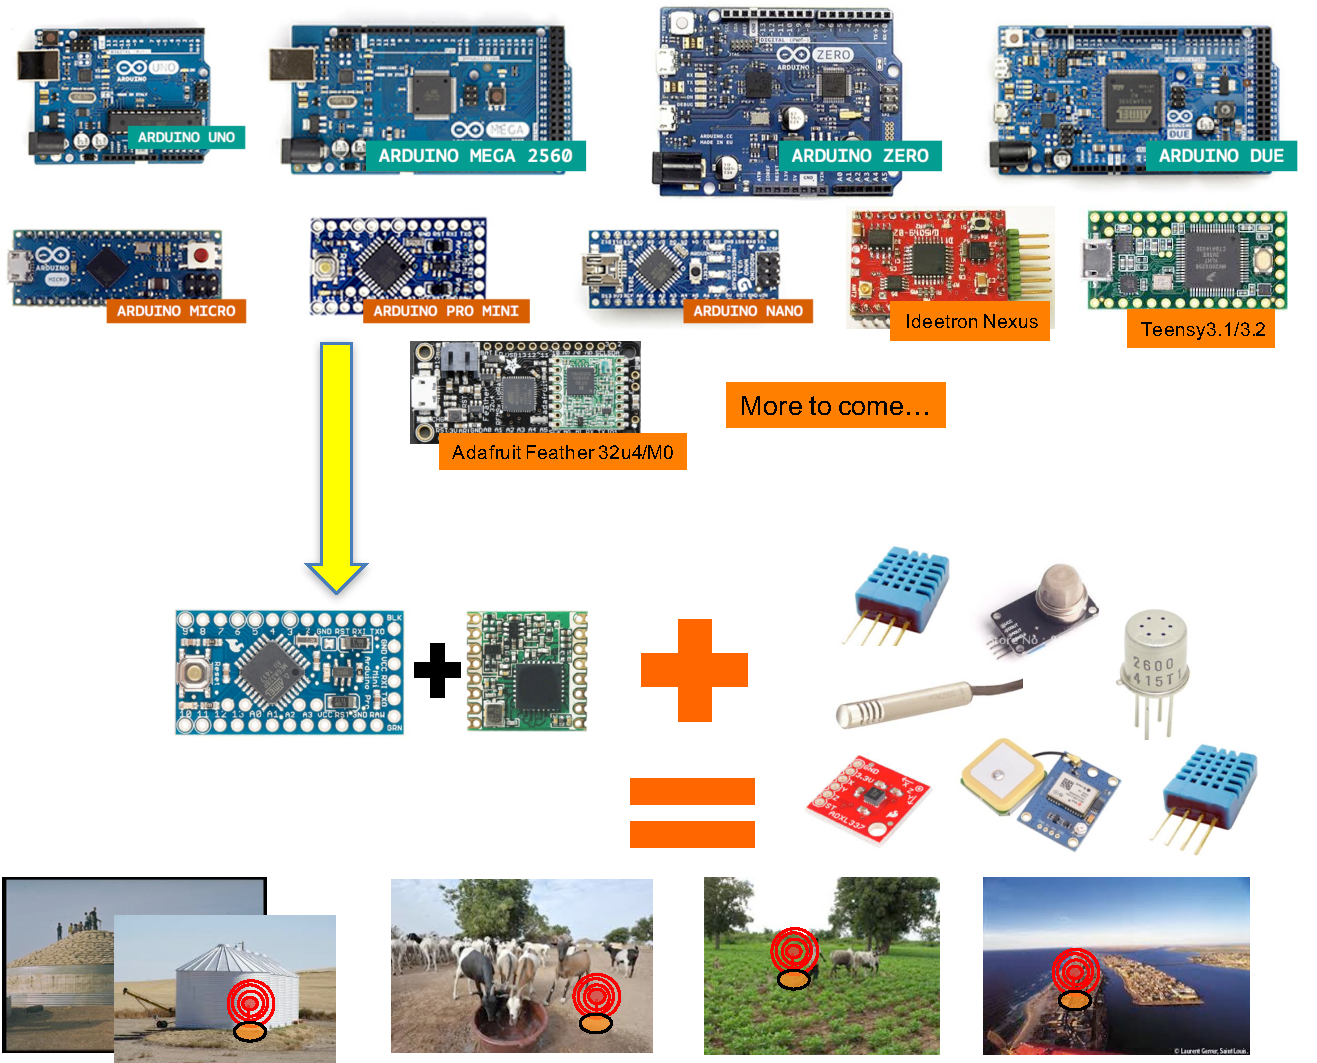
\includegraphics[width=.7\linewidth]{figures/generic-iot}   
\caption{Generic low-cost IoT hardware}   
\label{figure-generic-iot}  
\end{figure} 

\vspace{-0.5cm}
The Arduino ecosystem is large and proposes various board models, from large and powerful prototyping boards to smaller and less energy-consuming boards for final integration purposes as illustrated in Figure \ref{figure-generic-iot}.
For instance, the small form factor Arduino Pro Mini board based on an ATmega328 microcontroller has a high performance/price tradeoff and can be used to build a low-cost generic sensing IoT platform with LoRa long-range transmission capability for about 7 euro: 2 euro for the Arduino and 5 euro for the radio module! Integration of these generic IoT becomes straightforward and the Arduino Pro Mini is available in the 3.3v \& 8MHz version for much lower power consumption, offering the possibility of running for more than a year on 4 AA regular batteries as illustrated in Figure \ref{figure-easy-integration}.


\begin{figure}[H] 
\centering  
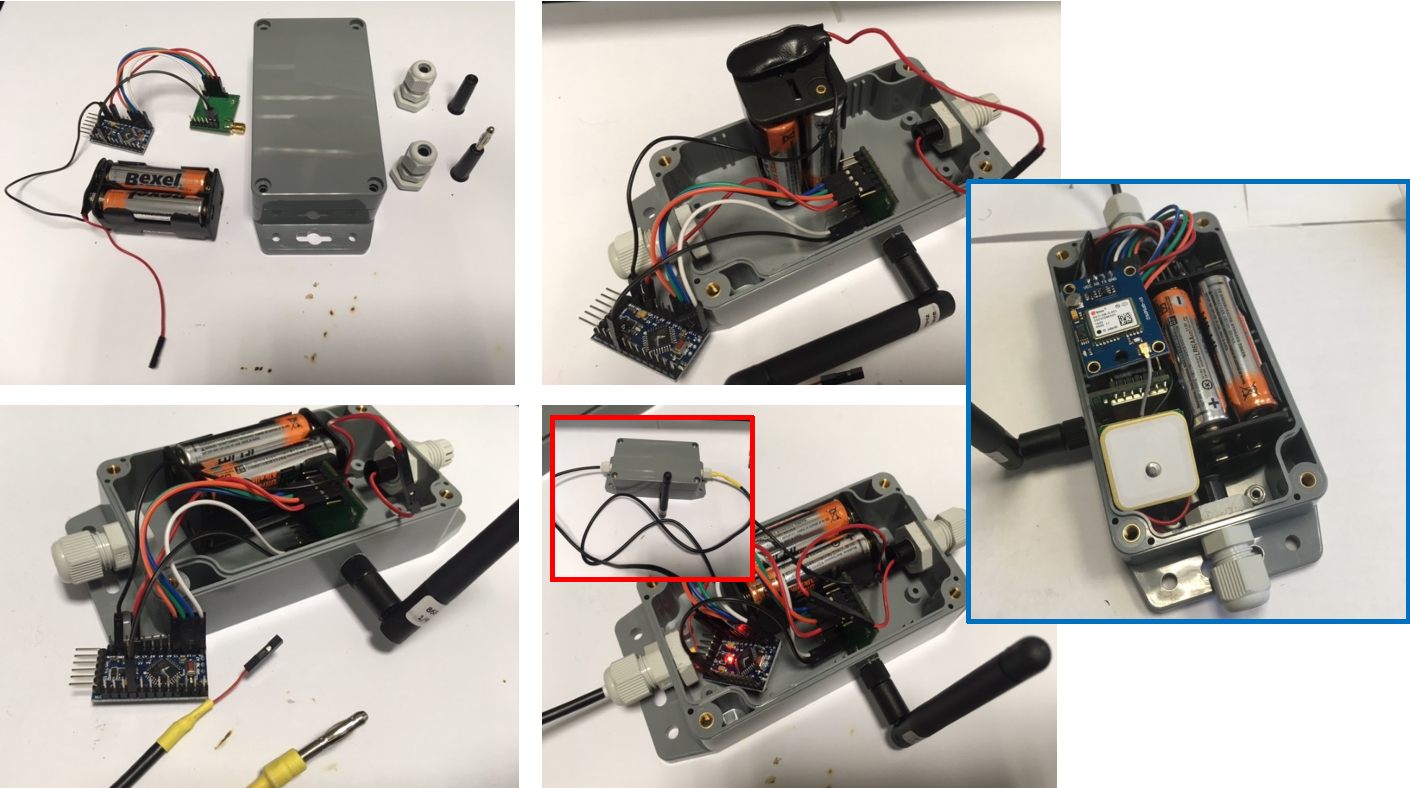
\includegraphics[width=.8\linewidth]{figures/easy-integration}   
\caption{Easy integration with DIY approach for maximum appropriation}   
\label{figure-easy-integration}  
\end{figure} 

\vspace{-0.5cm}
It is expected that this availability of low-cost DIY IoT will create a tremendous uptake of the technology on a large-scale, for a large variety of applications, including those from developing countries as even a limited deployment of IoT devices can have huge impacts.


\subsection{Handling IoT data}

A complete IoT system should be able to leverage big data technique for storing, processing, and analysing data.
Such a technique is Hadoop MapReduce \cite{hadoop}.
It is a scalable data analysis and processing tool.
Apache Spark \cite{spark} is a different data analytics system.
With in-memory capability, it claimed to be faster than MapReduce up to a hundred times.
Apache Flume \cite{flume} is a distributed, reliable service for collecting, aggregating and moving large amounts of streaming data.
Apache Kafka \cite{kafka} is a high-throughput, distributed, publish-subscribe messaging system.
With Kafka, data can be consumed by multiple applications.
Orion Context Broker \cite{orion} provides a publish-subscribe mechanism for registering context elements and managing them through updates and queries.
To this end, Apache Flink \cite{flink} is a streaming data flow engine (realtime stream processing) that provides data distribution, communication and fault-tolerance.


However, there are currently several new approaches based on Platform as a Service (PaaS) offering more flexible IoT services with data processing capacity inspired from Big Data techniques and the possibility to manage storage cloud in both local and global manner.
The idea of extending the PaaS approach to IoT is to propose a platform dedicated to IoT developers that can reduce the time-to-market for an application by cutting the development costs.
Big Data techniques enable the processing of huge amount of data produced by sensors.
These techniques allow creating actionable information and knowledge out of raw data.
To this end, the local and global clouds address the intermittent connection challenge: when Internet is not available, the user can still access some IoT functionalities from the local Cloud.


\begin{figure} 
\centering  
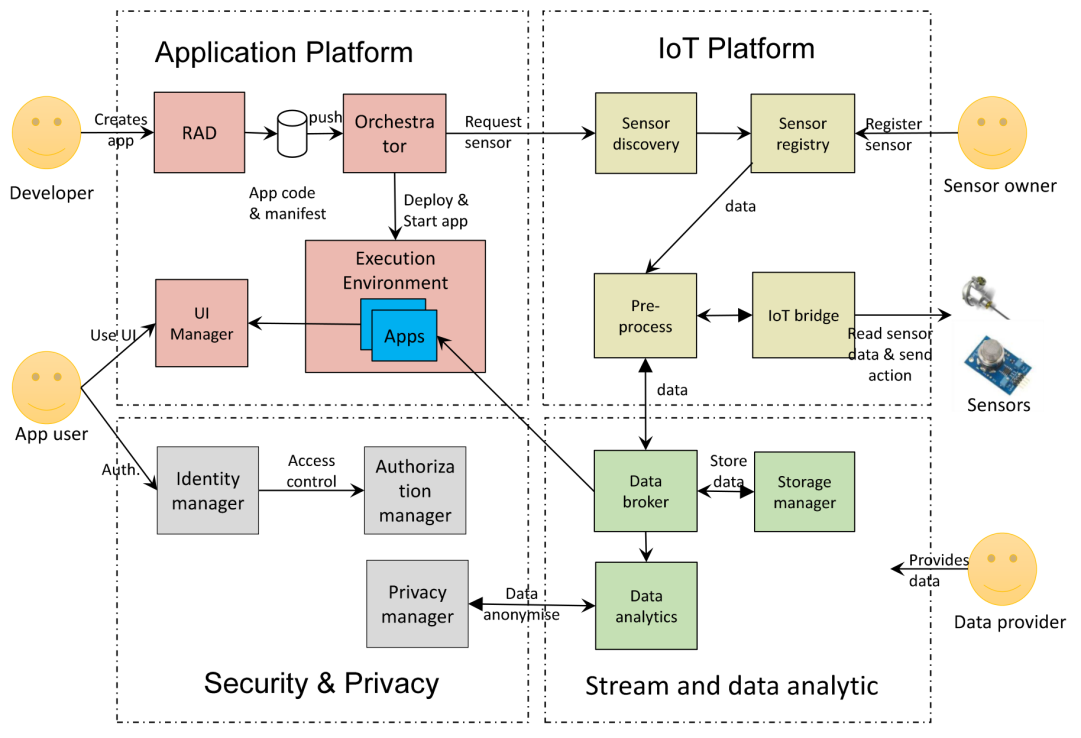
\includegraphics[width=.9\linewidth]{figures/GlobalArch}   
\caption{IoT platform architecture}   
\label{figure-globalarch}  
\end{figure} 

\vspace{-0.5cm}
Figure \ref{figure-globalarch} presents a typical architecture of such an IoT platform.
It shows the four main functional domains: Application Platform, IoT Platform, Security and Privacy, and Stream \& Data Analytic.
The Application Platform involves the development of the application itself and its deployment in the Cloud and in the Gateway.
For this purpose, a rapid application development (RAD) tool can be used, such as Node-Red.
A user can provide the source code of the application, together with its manifest.
The manifest file describes the application's requirements in terms of RAM, CPU, disk and also data sources (e.g.
real sensors, Internet sources), big data processing engines (e.g Flink, Hadoop), and application deployment (in the Cloud and in the IoT Gateway).


In this kind of approach and architecture, the application source code, together with the manifest, is pushed to the Cloud platform by the user.
The orchestrator component will read the manifest and trigger the compilation of the application.
It will then deploy the application in the Cloud Execution Environment.
It will also instantiate the services needed by the application, as described in the manifest.
The last task of the orchestrator is to request the sensor and data sources connections from the IoT components.
The sensor discovery module will be in charge of retrieving a list of sensors that matches the manifest description.
On the left side of the diagram, sensor owners can register their sensors with the platform.
External data sources such as Internet APIs can also be connected directly to data broker.
The sensors selected for each application will deliver their data to data broker, through the IoT bridge and pre-processor.
This last component is in charge of managing the connection and configuration of the sensors.
In addition, it will contain the routines for pre-processing of data, such as cleaning, extrapolating, aggregating and averaging.
Historical data can be stored using the Storage manager.


\section{The WAZIUP IoT platform}
\label{platform}

\subsection{Motivations and rationals}

While developed countries are discussing about massive deployment of IoT, developing countries are still far from being ready to enjoy the full benefit of IoT.
They face many challenges, such as the lack of infrastructure and the high cost of platforms with increasing complexity in deployment.
At the same time, it is urgent to promote IoT worldwide and not only for developed countries market.
The WAZIUP project will contribute by reducing part of the technology gap.
WAZIUP is focusing particularly in deploying IoT and Big Data platform for sub-saharan African countries as it is funded under the H2020 EU call for EU-Africa cooperation but many of its core propositions target developing countries is general.


The challenges of deploying a low-cost IoT, Big Data, and Cloud platform for developing countries will be tackled using an open IoT-Big Data Platform with affordable sensors connected through an Iot-Cloud open platform.
The technical functionalities encompassed by the platform will be a cloud-based real-time data collection combined with analytics and automation software, an intelligent analytics of sensor and device data, an integration to third parties platforms and a Platform-as-a-Service provider.


\subsection{Architecture overview and implementation}

The WAZIUP IoT platform (www.waziup.io) follows the flexible IoT platform illustrated previosuly in Figure \ref{figure-globalarch}.
The open source platform has been implemented with state of the art technology and there is a GitHub repository at https://github.com/Waziup/Platform.
It is the main repository for platform developers as well as application developer, being open it is accessible to everybody.
The real-world WAZIUP IoT platform implementation is further illustrated in Figure~\ref{fig-implem} which shows the WAZIUP cloud platform stack and its connection to IoT gateways through data broker (such as Orion Context Broker).


\begin{figure}[H] 
\centering  
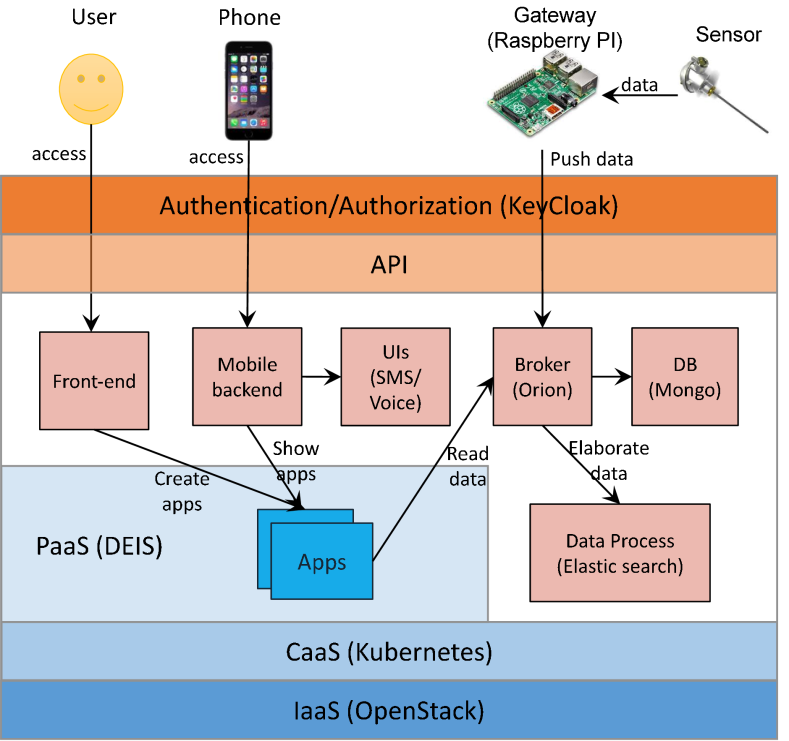
\includegraphics[width=.7\linewidth]{figures/CloudServicesArchitecture.png}   
\caption{Global overview of WAZIUP Cloud platform, and services}
\label{fig-implem}  
\end{figure}

\vspace{-0.5cm}
The role of each component is presented, together with the technology selected in parenthesis.
The WAZIUP IoT platform uses three distinct Cloud layers (in blue in the figure):

\begin{enumerate}
  \item Infrastructure as a Service (IaaS),    
  \item Container as a Service (CaaS),    
  \item and finally Platform as a Service�� (PaaS).

\end{enumerate}

The first layer is provided by {\tt OpenStack} \cite{openstack}.
Its main role is to provide Virtual Machines (VMs) that run the full platform.
This layer is fundamental because most of Cloud vendors (Amazon, Rackspace) use VMs as basic selling units.
The second layer is provided by {\tt Kubernetes} \cite{kubernetes}.
The role of this layer is to provide and serve containers, such as Docker containers, to WAZIUP services and applications.
The containers provide light-weight and ultra-fast virtualization for applications and micro-services.
The containers themselves are running inside the VMs.
The third and final Cloud layer is provided by {\tt Deis} \cite{deis}.
It provides services to developers, such as compiling and deploying of an application.
All the applications pushed by the users will be compiled with {\tt Deis} and hosted in containers on {\tt Kubernetes}.


Both Authentication and Authorization management is realized by {\tt Keycloak} \cite{keycloak} (e.g.
access the dashboard, access to the platform).
Users' applications (Web, mobile) and external components (e.g.
IoT gateway) need to go through an API server.
The API server exposes a common API for all the services of the WAZIUP platform and each endpoint of the API server is secured with {\tt Keycloak}.
In addition, through the dashboard and APIs the user can access only to sensors that are authorized for him.
This is enforced by {\tt Keycloak} authorization layer.


Mobile phones are used to interfaces with the SMS and voice commands component.
This component allows WAZIUP applications to send SMS and voice notifications to the users.


\subsection{Local and global clouds}

The WAZIUP IoT platform defines two different types of Clouds: the local Cloud and the global Cloud.
A local Cloud is an infrastructure able to deliver services to clients in a limited geographical area.
The local Cloud replicates some of the features provided by the traditional Cloud.
It is used for clients that may not have a good access to the traditional Cloud, or to provide additional processing power to local services.
In order for such an infrastructure to be considered as a local Cloud it must support a virtualization technology.
In the case of the WAZIUP IoT platform, the local Cloud comprises the end-user or service provider's personal computer and IoT Gateway.


\begin{figure}[H] 
\centering  
\includegraphics[width=.7\linewidth]{figures/localglobalcloud}   
\caption{Waziup local and global deployment}
\label{fig-localglobalcloud}  
\end{figure}

\vspace{-0.5cm}
The global Cloud, on the other end, is based on "backbone infrastructure" which increases the business opportunities for service providers and allows services to access a virtually infinite amount of computing resources.
In order for such an infrastructure to be considered as a global Cloud it must support a virtualization technology and be able to host the global cloud components of the WAZIUP architecture.


One of WAZIUP innovative approach to take into account developing countries' constraints is to extend the PaaS concept to the local Cloud.
On the left part of Figure \ref{fig-localglobalcloud}, the application is designed by the developer, together with the manifest file.
It is pushed on the WAZIUP Cloud platform.
The orchestrator then takes care of compiling and deploying the application in the various Cloud execution environments.
Furthermore, the orchestrator drives the instantiation of the services in the Cloud, according to the manifest.
The manifest is also describing which part of the application need to be installed locally, together with corresponding services.
The local application can then connect to the gateway and collect data from the sensors.






\subsection{Data Management and Analytics Architecture}

The IoT Gateway (e.g.
LoRa gateway) pushes IoT sensors' data to the data broker which can distribute further to final applications on request.
The WAZIUP architecture integrates the FIWARE Orion data broker for providing current sensor values and {\tt ElasticSearch} \cite{elastic} to keep the history (time series) of sensor values.
An ElasticSearch Feeder service is responsible for transferring data (current sensor values) from Orion to ElasticSearch (for historical record keeping).


ElasticSearch Feeder is written in NodeJS.
It accesses Orion and ElasticSearch through their REST APIs.
It allows transferring data from Orion to ElasticSearch either in a periodic manner (e.g.
every 5 minutes) or by subscription when data are recorded in ElasticSearch only if they change in Orion.
The ElasticSearch Feeder is configured by specifying a set of tasks, where each task defines the Orion'��s service path along with sensor' attributes and maps it to an ElasticSearch'��s index.
A commented example of the configuration is shown below.
The configuration is provided in YAML for 2 soil moisture devices ({\tt WS\_FARM1\_Sensor2} and {\tt WS\_FARM1\_Sensor3}) deployed in {\tt FARM1}.
Each device has 2 soil moisture physical sensors that provide 2 reading of soil moisture level at different depths ({\tt SM1} and {\tt SM2}) and will periodically send data string formatted as follows: {\tt SM1/554/SM2/345}.


\begin{verbatim}
# Defines the HTTP endpoint for subscriptions
endpoint:
  id: feeder1
  url: http://feeder
  host: 0.0.0.0
  port: 8000
# Defines the default ElasticSearch connection settings.

elasticsearch:
  host: elasticsearch
  port: 9200
# Defines the default Orion connection settings.

orion:
  uri: http://broker
# Defines (multiple) tasks.

- trigger: subscription
#  Specifies task-level Orion settings
  orion:
    service: waziup
    servicePath: /FARM1/TESTS
#  Specifies task-level Elasticsearch settings
  elasticsearch:
    index: test
#  Specifies the filter over the sensors discovered.

  filter:
#  If set, only entities listed below will be considered.

    ids:
    - WS_FARM1_Sensor2
    - WS_FARM1_Sensor3
#  If set, only attributes listed below will be considered.

    attributes:
    - SM1
    - SM2
\end{verbatim}

\subsection{Applications Platform Architecture}

WAZIUP vision is to make it easy for IoT developers to develop new applications, dashboards and services.
With WAZIUP APIs Server model, several generic proxy APIs services are developed, such as for Security (KeyCloak proxy API), Data Management (Orion proxy API), Data Analytics (ElasticSearch proxy API), etc.
These APIs may be developed as part of WAZIUP APIs Server, or as separate Service APIs that are just proxy APIs calling the respective service APIs.
Figure \ref{fig-app} illustrates this concept to create application templates.


\begin{figure}[H]  
\centering  
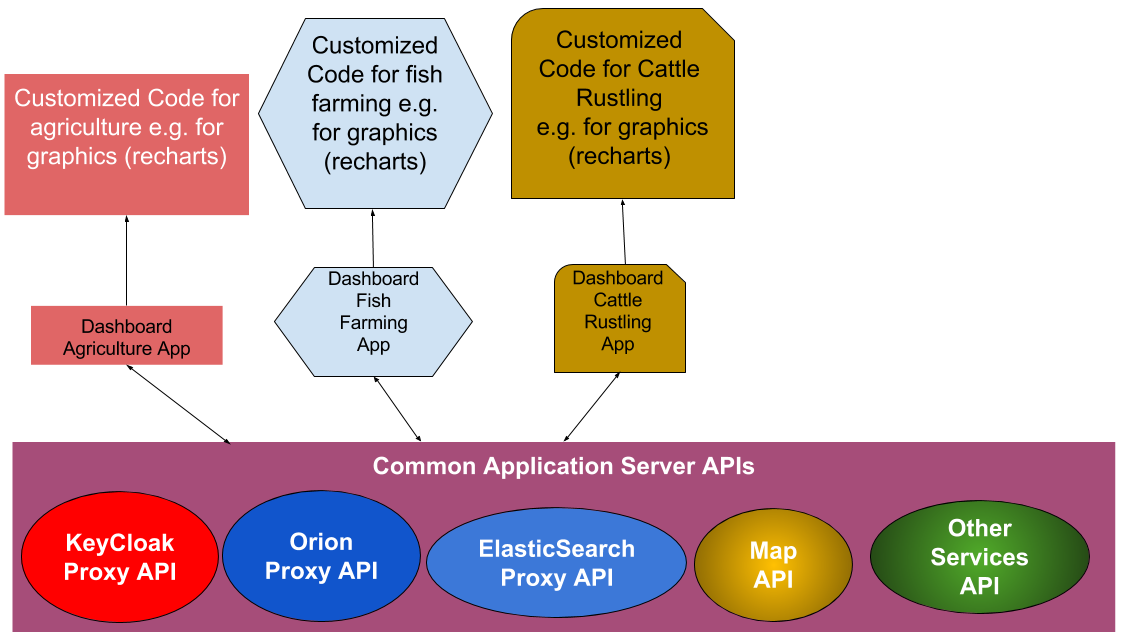
\includegraphics[width=.68\linewidth]{figures/AppArchitecture.png}   
\caption{A global view of WAZIUP Application Template platform}
\label{fig-app}
\end{figure}

\vspace{-0.5cm}
This approach is also taken at the Dashboard level where Application Development templates for IoT developers are provided to develop customized end-user applications.
These APIs will be developed as a NodeJS server.
For instance, instead of contacting the Orion broker in the client Dashboard, the Orion API of WAZIUP Server API is called to get the list of sensors, sensors data, subscriptions, etc.
This approach will make it easier for developers to develop new dashboards having in place those that are already developed and tested on top of WAZIUP Services.
Figure \ref{fig-dashboard} shows the dashboard developed for the WaterSense project in Pakistan (optimization of maize crop irrigation) using the WAZIUP framework.
Figure \ref{fig-sensor-data} shows {\tt WS\_FARM1\_Sensor2}'s historical data.


\begin{figure}[H]  
\centering  
\includegraphics[width=.73\linewidth]{figures/dashboard} 
\caption{A customized dashboard application for the soil moisture scenario}
\label{fig-dashboard}
\end{figure}

\vspace{-1cm}
\begin{figure}[H]  
\centering  
\includegraphics[width=.73\linewidth]{figures/sensor-data}
\caption{Historical data from sensor device}
\label{fig-sensor-data}
\end{figure}

\subsection{Service orchestration and resources provisioning}

The WAZIUP IoT platform offers mechanisms that autonomously analyze application requirements, user preferences and Cloud resources and accordingly decide upon the most appropriate deployment of services.
The most appropriate deployment must achieve the best balance between system performance, quality of service and cost.
In this context, services may be decomposed into smaller components, based on the current situation and information on data sources, in order to be migrated and executed in a local Cloud, near the data sources, following the Hadoop maxim "Moving Computation is Cheaper than Moving Data".
Alternatively, services may be deployed and executed in the global Cloud.
Furthermore, this mechanism will facilitate the notion of "Everything as a Service", and attached gateway to host and process services on-demand, by means of service migration instead of being limited to predefined services.
The local IoT Gateway may act as part of a local Cloud on an on-demand basis in coordination with the global Cloud, provided that the local Cloud has sufficient resources to process and execute the service.


%The platform used a model that allows the service to be analyzed and decomposed into a certain number of sub-components according to application requirements, user preferences including privacy constraints, policies, system state and data sources location.
The service sub-components are then migrated to either local Clouds, to be computed near the data sources (e.g., sensors) or into the global Cloud, to take advantage of the extensive computing power and storage available.
The optimal distribution is decided with the aim of achieving the best balance between overall system performance (network traffic, computing load), quality of services (prompt and accurate delivery of service result) and service costs.


\subsection{Platform Security Architecture}

Figure \ref{fig-services} illustrates WAZIUP services architecture in more details.
The access to different WAZIUP services is performed by the WAZIUP APIs server (Dashboard API Server in Figure \ref{fig-services}.


\vspace{-0.5cm}
\begin{figure}[H]
\centering
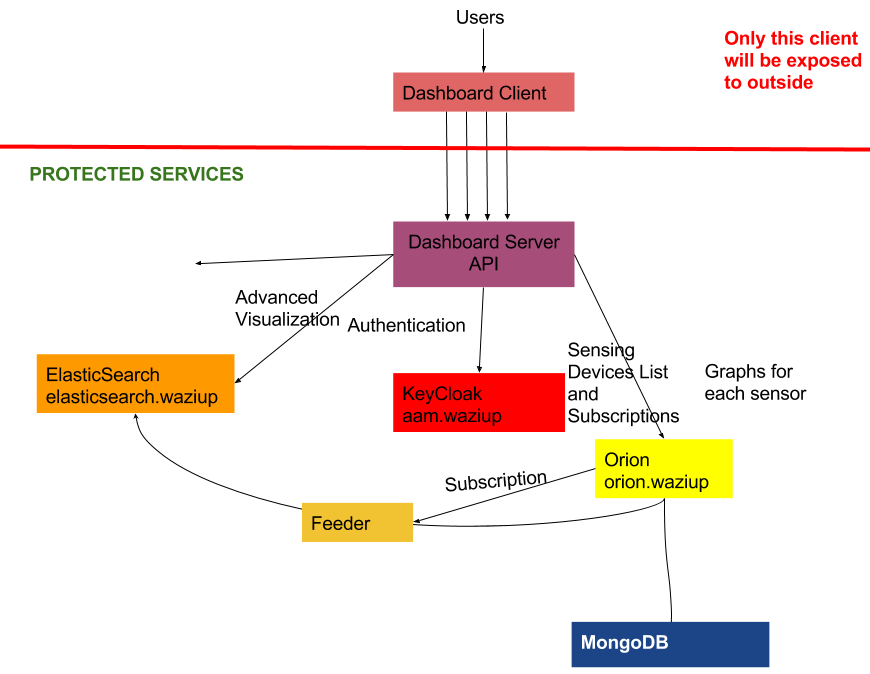
\includegraphics[width=.6\linewidth]{figures/ServicesArchitecture.png}
\caption{Detailed view of WAZIUP Cloud platform, and services architecture}
\label{fig-services}
\end{figure}

\vspace{-0.5cm}
The APIs server acts as a gateway placed in the demilitarized zone between the Internet and the internal network with WAZIUP services.
WAZIUP APIs server provides public endpoints for the internally hosted services and proxies to them.
All these services will not provide any Ingress to outside world.
APIs Server can communicate with all {\tt Kubernetes} internal services.
And can respond to Client queries about different services.
Thus, APIs Server will act as a proxy to provide security for WAZIUP services.


Authentication is the first requirement in implementing security.
Users should be first identified by WAZIUP platform, then they can request access to different resources, i.e.
authorization.
WAZIUP APIs server takes care of the authentication and authorization of incoming requests from the Internet.
Authentication is performed with {\tt Keycloak} server while authorization is done directly by the WAZIUP APIs server.

Depending on whether a service is accessed in an interactive manner (from a web-browser) or in a programmatic manner (directly from another service), WAZIUP APIs server provides two basic flows:

\begin{itemize}
\item Authentication for interactive use:
A user accesses a page (e.g.
through a Dashboard web client).
The browser sends a request to the APIs server.
The server finds out that client has not authenticated yet and redirects the client'��s browser to a login screen provided by {\tt Keycloak}.


\item Authentication for programmatic use (e.g.
from a sensor gateway):
A user generates (typically through some web-based client) an offline access refresh token.
The token is given to a device (e.g.
the sensor gateway) as a configuration parameter.
When the device wants to make a request, it contacts {\tt Keycloak} and requests an access token to be generated based on the refresh token.


\end{itemize}

Once the authentication is successful completed, the APIs server uses the access token to validate if the user/device has access to a particular resource.
For the sake of the authorization, every user has an attribute "permissions"�� (which is maintained by {\tt Keycloak}).
The attribute "permissions" attaches the the role of the user (admin, advisor or farmer) to resources (sensors, etc.) under a particular service path in Orion.
Examples of values of the "��permissions"�� attribute are listed below:

\begin{itemize}

\item "admin": admin access to anything regardless of the service path
\item "advisor: /FARM1; advisor: /FARM2" - advisor (i.e.
read-write access) to anything under /FARM1 and /FARM2 service paths
\item "farmer: /FARM1" - farmer at /FARM1
\item The roles can be combined, such that a user gets different roles at different service paths: "advisor: /FARM1; advisor: /FARM2; farmer: /FARM2; farmer: /FARM3" 

\end{itemize}

\section{Conclusion}
\label{sec:conclu}

With ICT technologies, developing countries can dramatically improve its productivity by enabling the rapid and cost-effective deployment of advanced and real-time monitoring.
However, deploying an IoT platform in developing countries comes with many challenges.
Among them, the most important are supporting low cost, low power, low bandwidth, and intermittent Internet.
Moreover, widely accessible communication means such as SMS and voice calls need to be supported to reach the maximum users.
In this article, we proposed an architecture and implementation for the IoT Big Data platform.
The concepts that underpin the platform are three: PaaS approach to IoT, data processing capacity inspired from Big Data techniques and, local and global Cloud.
The idea of extending the PaaS approach to IoT is to propose a platform dedicated to IoT developers that can reduce the time-to-market for an application by cutting the development costs.
The Big Data techniques enable the processing of the huge amount of data produced by sensors.
Those techniques allow creating actionable information and knowledge out of the raw data.
Finally, the local and global Clouds address the intermittent connection challenge: when Internet is not available, the user can still access some IoT functionalities from the local Cloud.


\section*{Acknowledgements}

This work has been carried out within the European project WAZIUP (H2020-ICT-687607).


\bibliographystyle{unsrt}
%\bibliography{reference,../../BIB/references}
\bibliography{reference}

\end{document}
